\begin{equation}
    \begin{gathered}
        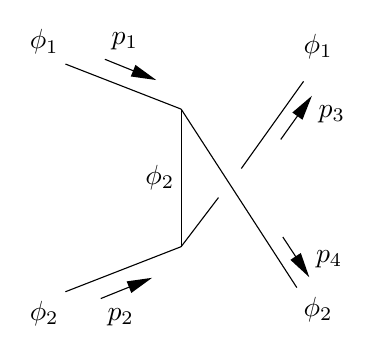
\begin{tikzpicture}[x=0.75pt,y=0.75pt,yscale=-1,xscale=1]
            %uncomment if require: \path (0,300); %set diagram left start at 0, and has height of 300
            
            %Straight Lines [id:da7163777291340228] 
            \draw    (268.45,215.45) -- (212.71,129.45) ;
            %Straight Lines [id:da9665644235261202] 
            \draw    (156.97,107.74) -- (212.71,129.45) ;
            %Straight Lines [id:da46015634659975735] 
            \draw    (175.98,105.45) -- (198.85,114.7) ;
            \draw [shift={(200.71,115.45)}, rotate = 202.02] [fill={rgb, 255:red, 0; green, 0; blue, 0 }  ][line width=0.08]  [draw opacity=0] (12,-3) -- (0,0) -- (12,3) -- cycle    ;
            %Straight Lines [id:da45449423366142727] 
            \draw    (274.54,124.69) -- (260.71,144.07) ;
            \draw [shift={(275.71,123.07)}, rotate = 125.54] [fill={rgb, 255:red, 0; green, 0; blue, 0 }  ][line width=0.08]  [draw opacity=0] (12,-3) -- (0,0) -- (12,3) -- cycle    ;
            %Straight Lines [id:da5734602899087693] 
            \draw    (212.71,129.45) -- (212.71,195.74) ;
            %Straight Lines [id:da3140324014019511] 
            \draw    (230.71,172.07) -- (212.71,195.74) ;
            %Straight Lines [id:da5132193871688708] 
            \draw    (156.97,217.45) -- (212.71,195.74) ;
            %Straight Lines [id:da42914137190821] 
            \draw    (173.98,220.74) -- (196.85,211.49) ;
            \draw [shift={(198.71,210.74)}, rotate = 517.98] [fill={rgb, 255:red, 0; green, 0; blue, 0 }  ][line width=0.08]  [draw opacity=0] (12,-3) -- (0,0) -- (12,3) -- cycle    ;
            %Straight Lines [id:da9510920186382812] 
            \draw    (273.35,208.78) -- (261.71,191.07) ;
            \draw [shift={(274.45,210.45)}, rotate = 236.68] [fill={rgb, 255:red, 0; green, 0; blue, 0 }  ][line width=0.08]  [draw opacity=0] (12,-3) -- (0,0) -- (12,3) -- cycle    ;
            %Straight Lines [id:da1510064266893021] 
            \draw    (271.71,116.07) -- (266.17,123.82) -- (241.71,158.07) ;
            
            % Text Node
            \draw (154.97,104.34) node [anchor=south east] [inner sep=0.75pt]    {$\phi _{1}$};
            % Text Node
            \draw (154.97,220.85) node [anchor=north east] [inner sep=0.75pt]    {$\phi _{2}$};
            % Text Node
            \draw (177.98,102.05) node [anchor=south west] [inner sep=0.75pt]    {$p_{1}$};
            % Text Node
            \draw (175.98,224.14) node [anchor=north west][inner sep=0.75pt]    {$p_{2}$};
            % Text Node
            \draw (210.71,162.59) node [anchor=east] [inner sep=0.75pt]    {$\phi _{2}$};
            % Text Node
            \draw (277.71,126.47) node [anchor=north west][inner sep=0.75pt]    {$p_{3}$};
            % Text Node
            \draw (276.45,207.05) node [anchor=south west] [inner sep=0.75pt]    {$p_{4}$};
            % Text Node
            \draw (270.45,106.34) node [anchor=south west] [inner sep=0.75pt]    {$\phi _{1}$};
            % Text Node
            \draw (270.45,218.85) node [anchor=north west][inner sep=0.75pt]    {$\phi _{2}$};
            \end{tikzpicture}            
    \end{gathered} \quad \begin{aligned}[t]
        &\eqqcolon \ii \mathcal{M}_{u2} = \frac{\ii}{(p_1 - p_4)^2 + \ii 0^+} ( \ii \lambda (p_4 - p_1) \cdot p_2) ( \ii \lambda (p_4 - p_1) \cdot p_4) \\
        &= - \ii \frac{\lambda^2 ((p_4 - p_1) \cdot p_2)((p_4 - p_1) \cdot p_4)}{u + \ii 0^+ }.
   \end{aligned}
\end{equation}